Consider a powergrid with $C$ consumers and $G$ generators. We are interested
in connecting each consumer to a single generator, but each generator has a
limited capacity and the consumer draws a certain amount of power from the
generator. A valid powergrid is built in such a way that all consumers are
serviced by a generator and that no generator is being overdrawn by too many
consumers. Although consumers and generators may be connected through a complex
network, we analyze the simple case where any consumer is able to attach to any
generator.

\begin{wrapfigure}{r}{0.5\textwidth}
   \begin{center}
      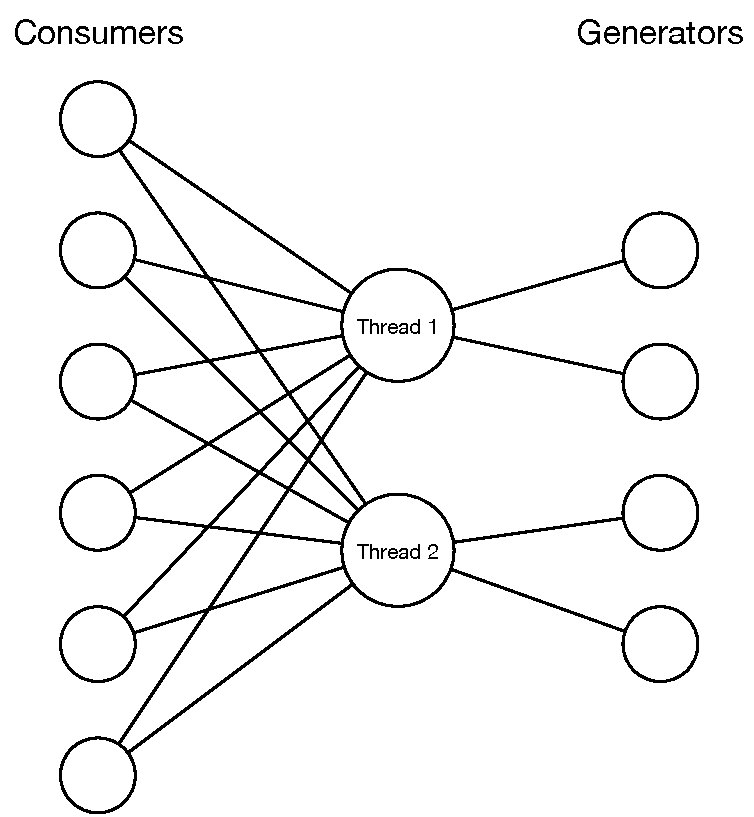
\includegraphics[width=1\linewidth]{figures/threads/powergrid.pdf}
   \end{center}
   \caption{Configuration of a powergrid with 6 consumers, 4
      generators and 2 threads, with each thread responsible for 2 generators.}
   \label{fig:threads:powergrid}
\end{wrapfigure}

A straightforward distributed implementation for the powergrid problem requires
that each consumer is able to connect to a any generator. Once a generator
receives a connection request, it may or may not accept it. If the generator has
no power available for the new consumer, it will disconnect from it and the
consumer must select another generator. This randomized algorithm works but may
take a long time to converge, depending on the amount of power available in the
generators. Figure~\ref{code:threads:powergrid} shows the LM code for this
solution. Consumer and generators node types are declared in
lines~\ref{line:threads:pg_decl1}-\ref{line:threads:pg_decl2} using the
\code{node} declaration, allowing us to have different predicates for consumers
and predicates. The \code{generator} and \code{consumer} types become a subtype
of \emph{node}, that is, $consumer <: node$ and $generator <: node$.  These
subtypes allow us to declare initial facts that only apply to either the
\code{consumer} or \code{generator} subtype.

All consumers start with a \code{reconnect} axiom that is used in
lines~\ref{line:threads:pg_connect1}-\ref{line:threads:pg_connect2} in order to
randomly select a generator from list \code{L}. Afterwards, the generator
receives a \code{connect} fact which is used in
lines~\ref{line:threads:pg_gen1}-\ref{line:threads:pg_gen2} when the generator
has enough power for the new consumer. When there is not enough power
(\code{Used + Power > Total}), the generator disconnects the consumer in
lines~\ref{line:threads:pg_fail1}-\ref{line:threads:pg_fail2}. Note that each
generator mantains a \code{fail} fact that counts the number of times the
consumers have failed to connected. If there is too many failures, then the
generator decides to disconnect one consumer already connected in
lines~\ref{line:threads:pg_recon1}-\ref{line:threads:pg_recon2}, allowing for
different combinations to happen.

\begin{figure}[h!]
\begin{Verbatim}[numbers=left,fontsize=\scriptsize,commandchars=*\#\&]
node generator.*label#line:threads:pg_decl1&
node consumer.*label#line:threads:pg_decl2&
type linear capacity(generator, int Total, int Used).
type linear connected-to(generator, consumer, int).
type linear connected-to-list(generator, list consumer).
type power(consumer, int).
type linear disconnected(consumer).
type linear connected(consumer, generator).
type generators(consumer, list generator).
type linear fails(generator, int).
type linear random-reconnect(generator).
type linear reconnect(consumer).
type linear connect(generator, consumer, int).
type linear disconnect(consumer, generator).

connected-to-list(G, []).  fails(G, 0).
disconnected(C).  reconnect(C).  !generators(C, all-generators).

fails(G, Fails), Fails > maxfails*label#line:threads:pg_recon1&
   -o random-reconnect(G).

capacity(G, Total, Used), random-reconnect(G),
connected-to-list(G, L), L <> [], C = nth(L, randint(length(L))),
connected-to(G, C, Power)
   -o fails(G, 0), capacity(G, Total, Used - Power),
      connected-to-list(G, remove(L, C)), disconnect(C, G).

capacity(G, Total, Used), random-reconnect(G)
   -o capacity(G, Total, Used), fails(G, 0).*label#line:threads:pg_recon2&

connect(G, C, Power), capacity(G, Total, Used),*label#line:threads:pg_gen1&
fails(G, Fails), connected-to-list(G, L), Used + Power <= Total
   -o capacity(G, Total, Used + Power),
      fails(G, max(Fails - 1, 0)), connected-to(G, C, Power),
      connected-to-list(G, [C | L]).*label#line:threads:pg_gen2&

connect(G, C, Power), capacity(G, Total, Used),*label#line:threads:pg_fail1&
Used + Power > Total, fails(G, Fails)
   -o capacity(G, Total, Used), disconnect(C, G),
      fails(G, Fails + 1).*label#line:threads:pg_fail2&

!generators(C, L), !power(C, Power),*label#line:threads:pg_connect1&
reconnect(C), disconnected(C),
G = nth(L, randint(num-generators))
   -o connected(C, G), connect(G, C, Power).*label#line:threads:pg_connect2&

disconnect(C, G), connected(C, G)
   -o disconnected(C), reconnect(C).
\end{Verbatim}
\caption{LM code for the regular powergrid program.}
\label{code:threads:powergrid}
\end{figure}

The issue with the distributed implementation presented in
Fig.~\ref{code:threads:powergrid} is that it lacks a global view of the problem,
which introduces inneficiencies and more communication between consumers and
generators. A better distributed algortihm will require more complicated
communication patterns between the nodes.  As we have seen before, thread local
facts are an excellent mechanism to introduce a global view of the problem
without complicating the original algorithm written in a declarative style. For
our solution, we will partition the set of generators $G$ among the threads in
the system and make each thread assume the ownership of its generators. The
thread can then process consumers with a global view over its set of generators,
allowing the immediate assignment iof consumers to generators.
Figure~\ref{fig:threads:powergrid} shows how a powergrid configuration is
re-configured to take into account the number of available threads.

The LM code using thread facts shown in Fig.~\ref{code:threads:powergridt} uses
4 thread predicates: \code{thread-connected-to} and
\code{thread-connected-to-list} assign consumers to the generators owned by the
thread; \code{thread-capacity} stores the capacity of the thread's generators;
and \code{thread-total-capacity} provides a capacity overview of the generators.
The program starts with the rule in
lines~\ref{line:threads:pgt_start1}-\ref{line:threads:pgt_start2} by moving
generators to their corresponding threads using \code{set-thread}. Once the
generator is executing on the proper thread, the rule in
lines~\ref{line:threads:pgt_moved1}-\ref{line:threads:pgt_moved2} is derived
with the \code{just-moved} coordination fact and the state of the thread is
initialized.  Consumers connect with the thread's generators with the rule in
lines~\ref{line:threads:pgt_con1}-\ref{line:threads:pgt_con2} by selecting the
first generator with enough power and then updating the state of the thread.
Otherwise, if the thread does not have a suitable generator, a generator is
randomly selected using the method shown before. For such cases, the thread
assigned with the selected generator will derive the rules in
lines~\ref{line:threads:pgt_gen1}-\ref{line:threads:pgt_gen2} and the thread
state is updated accordingly.

\begin{figure}[h!]
\begin{Verbatim}[numbers=left,fontsize=\scriptsize,commandchars=*\#\&]
type linear thread-connected-to(thread, generator, consumer, int).
type linear thread-connected-to-list(thread, generator, list consumer).
type linear thread-capacity(thread, generator, int, int).
type linear thread-total-capacity(thread, int, int).
type linear start(generator).

thread-total-capacity(T, 0, 0).
fails(G, 0).  disconnected(C).  reconnect(C).  !generators(C, all-generators).  start(G).

start(G), !generator-id(G, Id)*label#line:threads:pgt_start1&
   -o set-thread(G, Id % @threads).*label#line:threads:pgt_start2&

just-moved(G), capacity(G, Total, Used), thread-total-capacity(T, TotalCapacity, TotalUsed)*label#line:threads:pgt_moved1&
   -o thread-connected-to-list(T, G, []), thread-capacity(T, G, Total, Used),
      thread-total-capacity(T, Total + TotalCapacity, Used + TotalUsed).*label#line:threads:pgt_moved2&

fails(G, Fails), Fails > maxfails
   -o random-reconnect(G).

thread-capacity(T, G, Total, Used), thread-total-capacity(T, TotalCapacity, TotalUsed),
random-reconnect(G), thread-connected-to-list(T, G, L), L <> [], C = nth(L, randint(length(L))),
thread-connected-to(T, G, C, Power), NewUsed = Used - Power
   -o fails(G, 0), thread-capacity(T, G, Total, NewUsed),
      thread-total-capacity(T, TotalCapacity, TotalUsed - Power),
      thread-connected-to-list(T, G, remove(L, C)), disconnect(C, G).

random-reconnect(G) -o fails(G, 0).

connect(G, C, Power), thread-total-capacity(T, TotalCapacity, TotalUsed),*label#line:threads:pgt_gen1&
thread-capacity(T, G, Total, Used), fails(G, Fails), thread-connected-to-list(T, G, L),
NewUsed = Used + Power, NewUsed <= Total
   -o thread-capacity(T, G, Total, NewUsed),
      thread-total-capacity(T, TotalCapacity, TotalUsed + Power),
      fails(G, max(Fails - 1, 0)), thread-connected-to(T, G, C, Power),
      thread-connected-to-list(T, G, [C | L]).

connect(G, C, Power), thread-capacity(T, G, Total, Used), Used + Power > Total, fails(G, Fails)
   -o thread-capacity(T, G, Total, Used), disconnect(C, G), fails(G, Fails + 1).*label#line:threads:pgt_gen2&

!power(C, Power), reconnect(C), disconnected(C), thread-total-capacity(T, TotalCapacity, TotalUsed),*label#line:threads:pgt_con1&
TotalNewUsed = TotalUsed + Power, NewUsed <= TotalCapacity,
thread-capacity(T, G, Total, Used), thread-connected-to-list(T, G, ConnectList),
NewUsed = Used + Power, NewUsed <= Total
   -o connected(C, G), thread-capacity(T, G, Total, NewUsed),
      thread-connected-to-list(T, G, [C | ConnectList]), thread-connected-to(T, G, C, Power),
      thread-total-capacity(T, TotalCapacity, TotalNewUsed).*label#line:threads:pgt_con2&

!generators(C, L), !power(C, Power), reconnect(C), disconnected(C), G = nth(L, randint(num-generators))*label#line:threads:pgt_conn1&
   -o connected(C, G), connect(G, C, Power).*label#line:threads:pgt_conn2&

disconnect(C, G), connected(C, G)
   -o disconnected(C), reconnect(C).
\end{Verbatim}
\caption{LM code for the optimized powergrid program.}
\label{code:threads:powergridt}
\end{figure}

\clearpage
